\documentclass[]{article}

\usepackage{graphicx}
\usepackage{booktabs}
\usepackage{adjustbox}


% Title Page
\title{IE5202 Project 2 Report}
\author{Yang Xiaozhou, A0113538}


\begin{document}
\maketitle

\section{Data Exploration}

To visualize the linear relationship between target variable and the predictors, various scatter plots with regression lines are examined. In Figure \ref{fig:pairplot1}, it can be seen that essential features have weak positive features with target variable. However, among themselves, several features have strong positive correlation, as seen in Figure \ref{fig:jointplot1}, Figure \ref{fig:jointplot2} and Figure \ref{fig:jointplot3}.
%
\begin{figure}[hbtp]
	\centering
	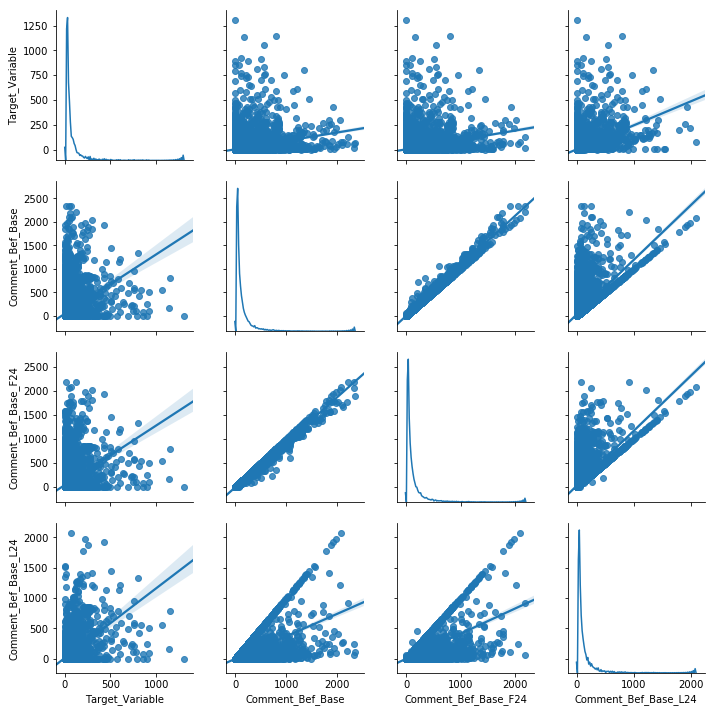
\includegraphics[width=0.6\columnwidth]{../Figures/pairplot1}
	\caption{Relationship between target variable and essential features.}
	\label{fig:pairplot1}
\end{figure}
%
%
\begin{figure}[hbtp]
	\centering
	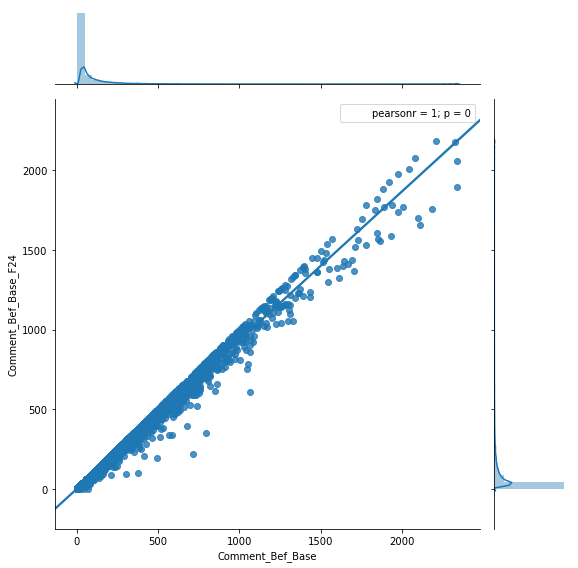
\includegraphics[width=.5\columnwidth]{../Figures/jointplot1}
	\caption{Comment before base time and comment before base time (first 24 hours).}
	\label{fig:jointplot1}
\end{figure}
%
%
\begin{figure}[hbtp]
	\centering
	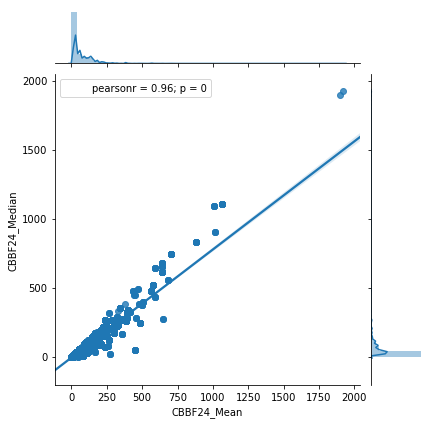
\includegraphics[width=.5\columnwidth]{../Figures/jointplot2}
	\caption{Comment before base time (mean of first 24 house) and comment before base time (median of first 24 hours).}
	\label{fig:jointplot2}
\end{figure}
%
%
\begin{figure}[hbtp]
	\centering
	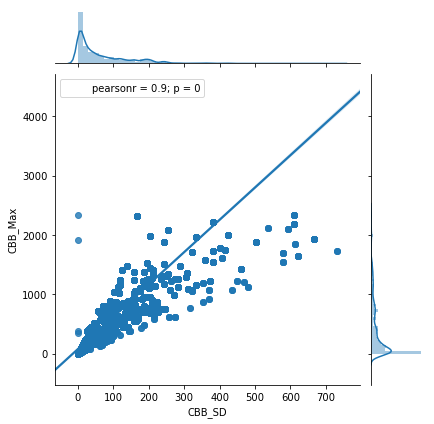
\includegraphics[width=.5\columnwidth]{../Figures/jointplot3}
	\caption{Comment before base time (standard deviation) and comment before base time (maximum).}
	\label{fig:jointplot3}
\end{figure}
%

While other variables do not show strong linear relationship with the target variable, the box-plot of Page Category (4) does show that the difference in page category have some influence on the target variable, see Figure \ref{fig:boxplot1}.
%
\begin{figure}[hbtp]
	\centering
	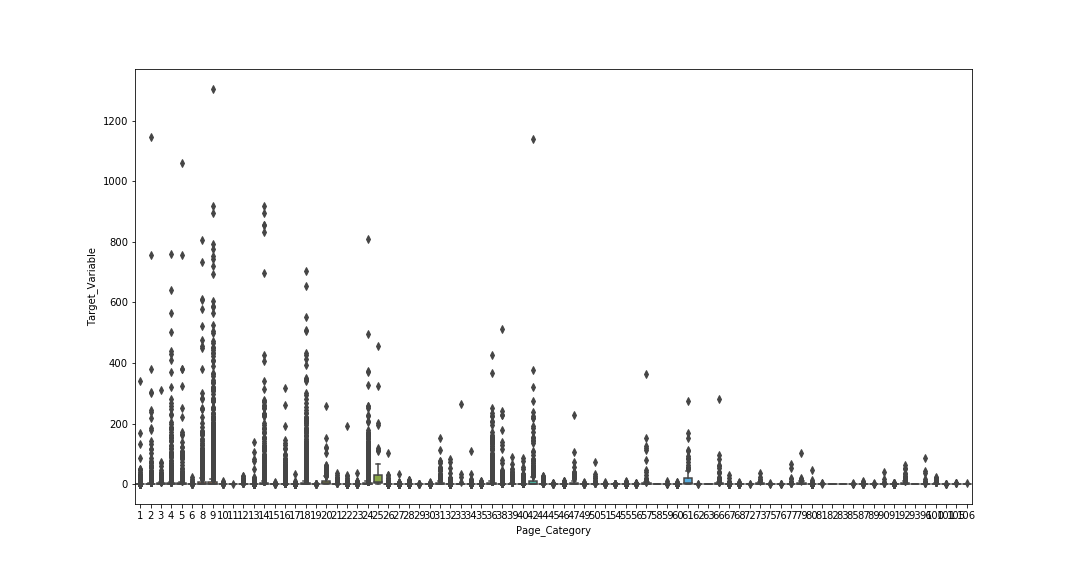
\includegraphics[width=1\columnwidth]{../Figures/box_page_cat}
	\caption{Boxplot of page category and target variable.}
	\label{fig:boxplot1}
\end{figure}
%

Another thing that is worth noting is the many variables, including the target variable empirically has the form of a power distribution that is heavily right-tailed. This can be seen in Figure \ref{fig:density}. 
%
\begin{figure}[hbtp]
	\centering
	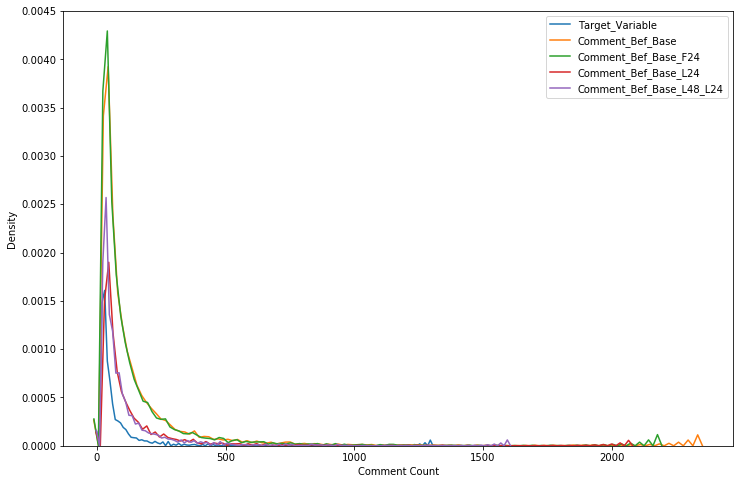
\includegraphics[width=1\columnwidth]{../Figures/density_plot}
	\caption{Emprical density of variables ensemble power distributions.}
	\label{fig:density}
\end{figure}
%



\section{Simple Regression Model}
\subsection{Model Building}
Without any interaction terms, the candidates used in this regression model is:
\begin{itemize}
	\item 12 Mean of comment count in last 24 hours
	\item 26 Maximum of comment difference between C2 and C3
	\item 31 Comment of the last 24 hours but before base time
	\item 33 Comment of the first 24 hours but before base time
	\item 34 Comment difference between C2 and C3
	\item 35 Time gap
\end{itemize}

Also, both the target variable and non-categorical variables are transformed through cube root function:
\begin{equation}
	\mathbf{Y} = \sqrt[3]{\mathbf{Y}}
\end{equation}
\begin{equation}
	\mathbf{X} = \sqrt[3]{\mathbf{X}}
\end{equation}

\subsection{Result}
Regression model summary can be found in Table \ref{tab:simple_summary} and the 10-fold cross-validation score can be found in Table \ref{tab:cv_result}.

\begin{table}
\begin{center}
	\begin{tabular}{lclc}
		\toprule
		\textbf{Dep. Variable:}          & Target Variable  & \textbf{  R-squared:         } &     0.679   \\
		\textbf{Model:}                  &       OLS        & \textbf{  Adj. R-squared:    } &     0.679   \\
		\textbf{Method:}                 &  Least Squares   & \textbf{  F-statistic:       } & 1.442e+04   \\
		\textbf{Date:}                   & Sat, 30 Sep 2017 & \textbf{  Prob (F-statistic):} &     0.00    \\
		\textbf{Time:}                   &     16:57:42     & \textbf{  Log-Likelihood:    } &   -41766.   \\
		\textbf{No. Observations:}       &       40949      & \textbf{  AIC:               } & 8.355e+04   \\
		\textbf{Df Residuals:}           &       40942      & \textbf{  BIC:               } & 8.361e+04   \\
		\textbf{Df Model:}               &           6      & \textbf{                     } &             \\
		\bottomrule
	\end{tabular}
	\begin{tabular}{lcccccc}
		& \textbf{coef} & \textbf{std err} & \textbf{t} & \textbf{P$>$$|$t$|$} & \textbf{[0.025} & \textbf{0.975]}  \\
		\midrule
		\textbf{Intercept}               &       1.3103  &        0.017     &    77.656  &         0.000        &        1.277    &        1.343     \\
		\textbf{Comment\_Diff\_C2\_C3}   &       0.0434  &        0.002     &    21.095  &         0.000        &        0.039    &        0.047     \\
		\textbf{CBBL24\_Mean}            &       0.2412  &        0.007     &    33.442  &         0.000        &        0.227    &        0.255     \\
		\textbf{Comment\_Diff\_Max}      &      -0.0490  &        0.003     &   -18.366  &         0.000        &       -0.054    &       -0.044     \\
		\textbf{Comment\_Bef\_Base\_F24} &       0.1302  &        0.005     &    28.297  &         0.000        &        0.121    &        0.139     \\
		\textbf{Time\_Gap}               &      -0.4748  &        0.005     &   -94.776  &         0.000        &       -0.485    &       -0.465     \\
		\textbf{Comment\_Bef\_Base\_L24} &       0.2573  &        0.005     &    47.253  &         0.000        &        0.247    &        0.268     \\
		\bottomrule
	\end{tabular}
	\begin{tabular}{lclc}
		\textbf{Omnibus:}       & 13471.617 & \textbf{  Durbin-Watson:     } &     1.847   \\
		\textbf{Prob(Omnibus):} &    0.000  & \textbf{  Jarque-Bera (JB):  } & 167947.876  \\
		\textbf{Skew:}          &    1.227  & \textbf{  Prob(JB):          } &      0.00   \\
		\textbf{Kurtosis:}      &   12.613  & \textbf{  Cond. No.          } &      41.9   \\
		\bottomrule
	\end{tabular}
\end{center}
\caption{OLS Regression Results - Simple Model}
\label{tab:simple_summary}
\end{table}

This regression model with 6 predictors yield an adjusted $R^2$ score of 0.679, which indicates that the model is not a strong representation of the relationship between the target variable and predictors. Since the F-statistic is large and the related p-value is very close to zero, there is strong evidence at 95\% significant level to reject the null hypothesis that none of the predictors need to be in the model. 

In the predictor table, coefficients of each predictor and the intercept value are reported. P-value of each of the predictor coefficients and the intercept is really close to 0 (reported as 0), this means that each of them have a value that is significantly different from 0 at 95\% significant level. 

Durbin-Watson statistic is 1.847, which is close to 2. This indicates insignificant level of autocorrelation in the residuals produced by this regression model. Also, the condition number here is 41.9, which may suggest that there is no strong collinearity between the covariates. However, upon further investigation, there is actually strong correlation between predictor 26 and 31, as shown in this scatter plot (Figure \ref{fig:predictor_corr_1}).  

\begin{table}
\centering
\begin{tabular}{lrr}
	\toprule
	{} &           \textbf{MAE} &       \textbf{MSE} \\
	\midrule
	0 &  4.242216 &   512.076063 \\
	1 &  4.380490 &   498.156699 \\
	2 &  4.994586 &  1001.783356 \\
	3 &  5.284419 &  1054.551894 \\
	4 &  4.618331 &   670.193012 \\
	5 &  5.210752 &  1228.869105 \\
	6 &  5.063661 &   820.874563 \\
	7 &  5.853072 &  1125.894034 \\
	8 &  4.385391 &   573.695776 \\
	9 &  5.127996 &  1223.085040 \\
	\textbf{Mean}  &   \textbf{4.916092} &   \textbf{870.917954} \\
	\bottomrule
\end{tabular}

\caption{Cross Validation Result}
\label{tab:cv_result}
\end{table}

To measure the prediction performance of the regression model, a 10-fold cross-validation technique is used to collect the result in Table \ref{tab:cv_result}. Mean score of AIC and BIC are smaller than that reported in the summary table by about 8000. This table also reports the mean absolute error (MAE) and mean square error (MSE), which measures the prediction performance of the model on unseen data. In my model selection process, however, adjusted $R^2$ is used as the selection criterion. 
%
\begin{figure}[hbtp]
	\centering
	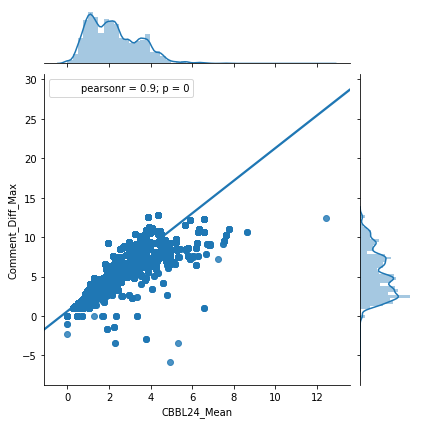
\includegraphics[width=.6\columnwidth]{../Figures/predictor_corr_1}
	\caption{Strong collinearity between two of the predictors.}
	\label{fig:predictor_corr_1}
\end{figure}
%

The QQ-plot plots the empirical quantiles of residuals and the quantiles of a standard normal distribution. In Figure \ref{fig:qq_plot_simple}, the sample quantiles do not form a straight line with the theoretical quantiles at both the left and right tails. This suggest that the normality assumption of the error term $\epsilon_i$ is violated. 
%
\begin{figure}[hbtp]
	\centering
	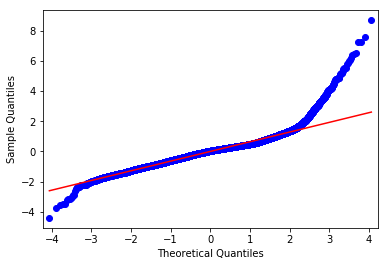
\includegraphics[width=.6\columnwidth]{../Figures/normality_check_simple}
	\caption{QQ-plot to check residual normality assumption.}
	\label{fig:qq_plot_simple}
\end{figure}
%

By examining the plot of studentized residuals and fitted values, several assumptions of the linear regression model could be verified. Figure \ref{fig:residual_plot_simple} shows the plot for this simple regression model. It seems that the residuals have a mean that is larger than 0 because more points lie above the zero line. Also, the variance of the residuals appear to increase with the fitted value, this suggests a violation of the constant variance assumption. Finally, there are plenty of residuals which have very large values (i.e. deviation from 0 with more than 3 standard deviations). This may indicate that the model is not adequate enough to fit the data well. 
%
\begin{figure}[hbtp]
	\centering
	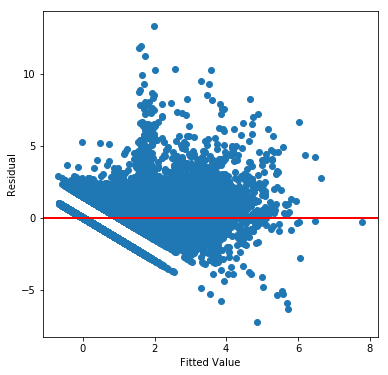
\includegraphics[width=.6\columnwidth]{../Figures/residual_plot_simple}
	\caption{Residual plot of the simple regression model.}
	\label{fig:residual_plot_simple}
\end{figure}
%


Two plots with partial regression are reported here for illustration with 
\begin{itemize}
	\item Post share count (Figure \ref{fig:prp_simple_1}), 
	\item Mean of comment count in last 24 hours (Figure \ref{fig:prp_simple_2}).
\end{itemize}
From both of the top left plots, it can be seen that the model tends to underestimate the target value as the bulk of fitted values lie below the target values. This may have to do with the fact that the target variable follows a heavily right-values empirical distribution. Both of the partial regression plots on the bottom left show a moderate positive relationship between the target variable and the individual predictor.  
%
\begin{figure}[hbtp]
	\centering
	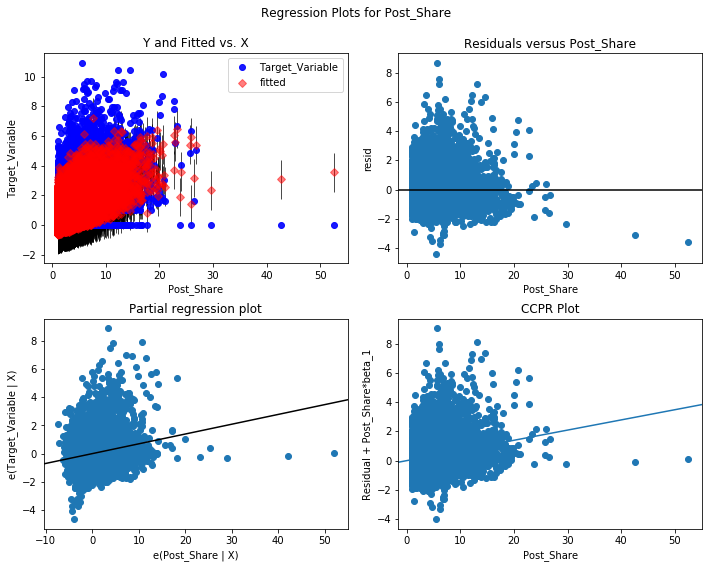
\includegraphics[width=1\columnwidth]{../Figures/prp_simple_1}
	\caption{Plots on predictor: Post share.}
	\label{fig:prp_simple_1}
\end{figure}
%
%
\begin{figure}[hbtp]
	\centering
	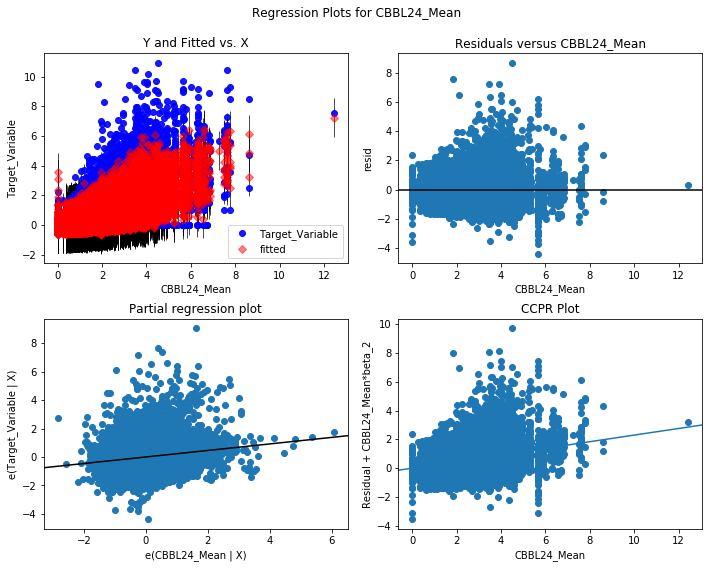
\includegraphics[width=1\columnwidth]{../Figures/prp_simple_2}
	\caption{Plots on predictor: Mean of comment count in last 24 hours.}
	\label{fig:prp_simple_2}
\end{figure}
%




\section{Complex Regression Model}
\subsection{Model Building}
In the complex regression model, interaction terms between two variables are added to the model. Based on the feature importance score (Figure \ref{fig:feature_imp}) extracted from an ensemble boosting tree regression model, 20 predictors with the highest importance are used as the basis for creating interaction terms. A complete list of the predictors can be found in Table \ref{tab:complex_predictors}. The same cube root transformation in simple regression model has been applied here as well. 
%
\begin{figure}[hbtp]
	\centering
	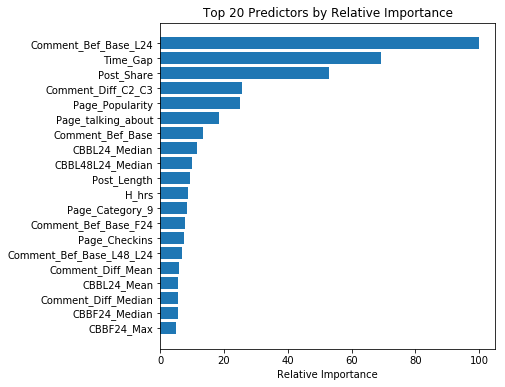
\includegraphics[width=.7\columnwidth]{../Figures/feature_importance}
	\caption{Top 20 predictors' relative feature importance generated from fitting a boosting tree regression model.}
	\label{fig:feature_imp}
\end{figure}
%
%
\begin{table}
\begin{center}
\begin{tabular}{ll}
	\toprule
	{} &                Predictors \\
	\midrule
	0  &      Comment\_Bef\_Base\_L24 \\
	1  &                  Time\_Gap \\
	2  &                Post\_Share \\
	3  &        Comment\_Diff\_C2\_C3 \\
	4  &           Page\_Popularity \\
	5  &        Page\_talking\_about \\
	6  &          Comment\_Bef\_Base \\
	7  &             CBBL24\_Median \\
	8  &          CBBL48L24\_Median \\
	9  &               Post\_Length \\
	10 &                     H\_hrs \\
	11 &           Page\_Category\_9 \\
	12 &      Comment\_Bef\_Base\_F24 \\
	13 &             Page\_Checkins \\
	14 &  Comment\_Bef\_Base\_L48\_L24 \\
	15 &         Comment\_Diff\_Mean \\
	16 &               CBBL24\_Mean \\
	17 &       Comment\_Diff\_Median \\
	18 &             CBBF24\_Median \\
	19 &                CBBF24\_Max \\
	\bottomrule
\end{tabular}
\end{center}
\caption{Predictors used for creating interaction terms.}
\label{tab:complex_predictors}
\end{table}
%

\subsection{Result}
Regression result for this model is reported in Table \ref{tab:complex_summary}. While the size of regression model has increased significantly from the simple model, the overall performance has also improved. Adjusted $R^2$ score is 0.799, hence the variation explained by the model is about 80\%, up from 67.9\% of the simple model. Test for all predictors are needed is successful with a close to zero p-value. Both AIC and BIC scores are smaller than those reported in the simple model. The Durbin-Watson statistic is still close to 2, which cause no alarm in residual autocorrelation. However, because of the high number of predictors deployed, the condition number of this model is very high. This suggests the presence of strong multicollinearity among certain predictors. This is not surprising, though, having seen strong correlation between predictors from the initial data exploration analysis. 

%
\begin{table}
\begin{center}
	\begin{tabular}{lclc}
	\toprule
	\textbf{Dep. Variable:}                                       & Target Variable  & \textbf{  R-squared:         } &     0.799   \\
	\textbf{Model:}                                               &       OLS        & \textbf{  Adj. R-squared:    } &     0.799   \\
	\textbf{Method:}                                              &  Least Squares   & \textbf{  F-statistic:       } &     1522.   \\
	\textbf{Date:}                                                & Sun, 01 Oct 2017 & \textbf{  Prob (F-statistic):} &     0.00    \\
	\textbf{Time:}                                                &     13:04:18     & \textbf{  Log-Likelihood:    } &   -32116.   \\
	\textbf{No. Observations:}                                    &       40949      & \textbf{  AIC:               } & 6.445e+04   \\
	\textbf{Df Residuals:}                                        &       40841      & \textbf{  BIC:               } & 6.538e+04   \\
	\textbf{Df Model:}                                            &         107      & \textbf{                     } &             \\
	\bottomrule
\end{tabular}

\begin{tabular}{lclc}
	\textbf{Omnibus:}       & 5945.914 & \textbf{  Durbin-Watson:     } &     1.888  \\
	\textbf{Prob(Omnibus):} &   0.000  & \textbf{  Jarque-Bera (JB):  } & 45015.854  \\
	\textbf{Skew:}          &   0.481  & \textbf{  Prob(JB):          } &      0.00  \\
	\textbf{Kurtosis:}      &   8.046  & \textbf{  Cond. No.          } &  2.98e+05  \\
	\bottomrule
	\end{tabular}
\end{center}
\caption{OLS Regression Results - Complex Model}
\label{tab:complex_summary}
\end{table}
%

Again, to accurately assess the prediction performance of the model to unseen data and prevent over-fitting on the available data, a 20-fold cross-validation technique is used to obtain performance metric values and the mean of these 20 values. They are reported in Table \ref{tab:cv_result_complex} and in a plot of the cross-validated mean square error (MSE) value (Figure \ref{fig:cv_mae_complex}). The mean value of MSE is 3.65893. 
%
\begin{table}
	\centering
\begin{tabular}{lrrrrr}
	\toprule
	{} &           \textbf{MAE} &       \textbf{MSE} \\
	\midrule
	0  &  2.902373 &   146.374018 \\
	1  &  3.560299 &   362.600952 \\
	2  &  3.768702 &   412.997428 \\
	3  &  3.051363 &   149.435547 \\
	4  &  3.548811 &   275.254989 \\
	5  &  3.942151 &   947.329354 \\
	6  &  3.410386 &   306.653846 \\
	7  &  4.319872 &   876.712590 \\
	8  &  2.993184 &   168.879596 \\
	9  &  3.731502 &   491.642907 \\
	10 &  4.235156 &  1032.601620 \\
	11 &  3.438691 &   217.428396 \\
	12 &  3.308620 &   295.118419 \\
	13 &  4.192867 &   391.431910 \\
	14 &  4.747604 &   906.253668 \\
	15 &  3.699576 &   215.585194 \\
	16 &  2.972562 &   206.520001 \\
	17 &  3.755930 &   478.474729 \\
	18 &  3.969618 &   829.406963 \\
	19 &  3.629519 &   215.318129 \\
	\textbf{Mean}  &  \textbf{3.658939} &   \textbf{446.301013} \\
	\bottomrule
\end{tabular}
	\caption{Cross Validation Result}
	\label{tab:cv_result_complex}
\end{table}
%
%
\begin{figure}[hbtp]
	\centering
	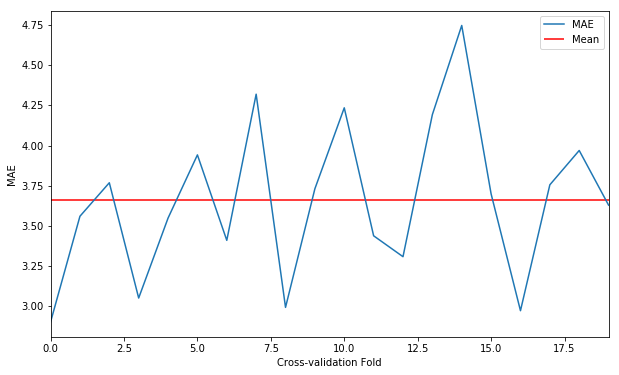
\includegraphics[width=1\columnwidth]{../Figures/cv_mae_complex}
	\caption{MAE score for 20-fold cross validation and their mean.}
	\label{fig:cv_mae_complex}
\end{figure}
%

The QQ-plot of residuals shows deviation of the points from the straight line at the tails. There seems to be slight improvement over the simple regression model. However, the obvious deviation suggests that the normality assumption of residuals is violated and the model might still need revision. 
%
\begin{figure}[hbtp]
	\centering
	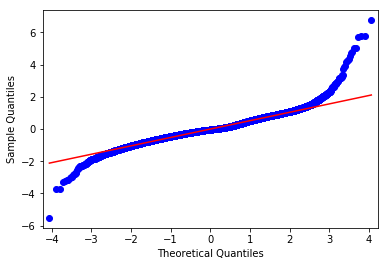
\includegraphics[width=.6\columnwidth]{../Figures/normality_check_complex}
	\caption{QQ-plot to check residual normality assumption.}
	\label{fig:qq_plot_complex}
\end{figure}
%

The plot of residuals against fitted value shows a similar pattern. While the number of large residuals decreased relative to the simple model, there are still many residuals outside the 3 standard deviations region. The variance of residuals seem to be non-constant as well, with smaller variance at the two ends of fitted value and larger variance in the middle. 
%
\begin{figure}[hbtp]
	\centering
	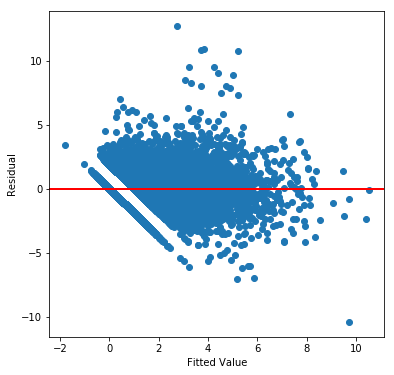
\includegraphics[width=.6\columnwidth]{../Figures/residual_plot_complex}
	\caption{Residual plot of the simple regression model.}
	\label{fig:residual_plot_complex}
\end{figure}
%

Plots of 5 individual predictors are also reported in Figure \ref{fig:prp_complex_1}, \ref{fig:prp_complex_2}, \ref{fig:prp_complex_3}, \ref{fig:prp_complex_4}, and \ref{fig:prp_complex_5}. From each of the top left plot, the issue of underestimation is not so severe now compared to the simple model. And the residuals seem to have mean 0 and constant variance for each of the individual predictor. One particular observation can be made from the 5 partial regression plots. The variance of residuals around value 0 of predictor regression error (x-axis) is significantly higher than at other values. 
%
\begin{figure}[hbtp]
	\centering
	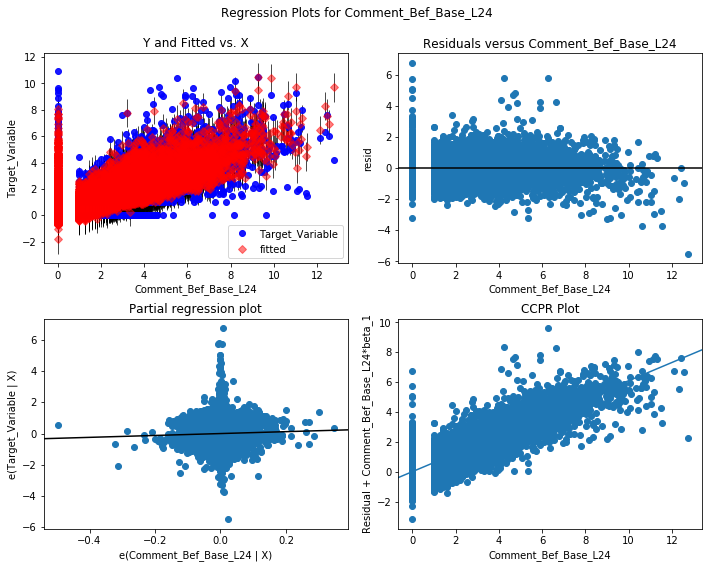
\includegraphics[width=.8\columnwidth]{../Figures/prp_complex_1}
	\caption{Plots on predictor: Comment count of last 24 hours before base time.}
	\label{fig:prp_complex_1}
\end{figure}
%
%
\begin{figure}[hbtp]
	\centering
	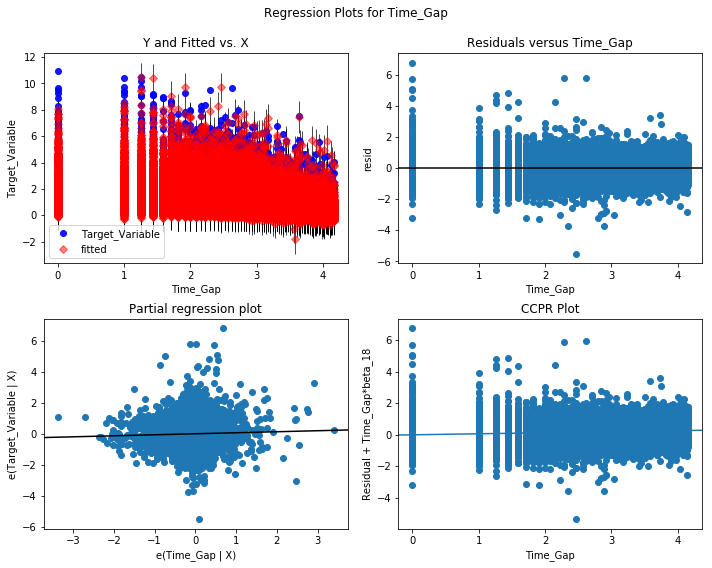
\includegraphics[width=.8\columnwidth]{../Figures/prp_complex_2}
	\caption{Plots on predictor: Time gap.}
	\label{fig:prp_complex_2}
\end{figure}
%
%
\begin{figure}[hbtp]
	\centering
	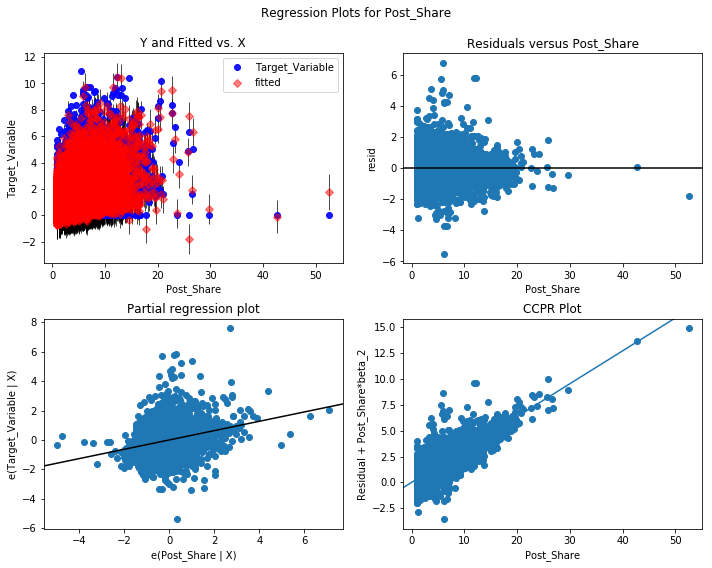
\includegraphics[width=.8\columnwidth]{../Figures/prp_complex_3}
	\caption{Plots on predictor: Post share count.}
	\label{fig:prp_complex_3}
\end{figure}
%
%
\begin{figure}[hbtp]
	\centering
	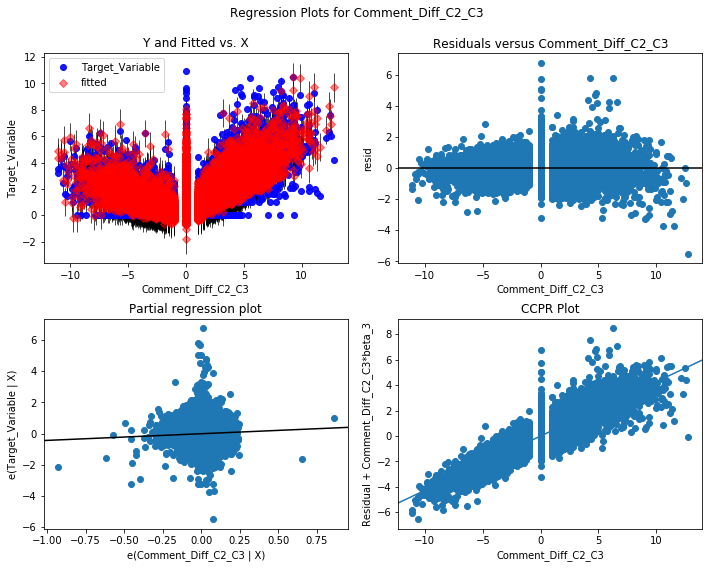
\includegraphics[width=.8\columnwidth]{../Figures/prp_complex_4}
	\caption{Plots on predictor: Comment count difference between C2 and C3.}
	\label{fig:prp_complex_4}
\end{figure}
%
%
\begin{figure}[hbtp]
	\centering
	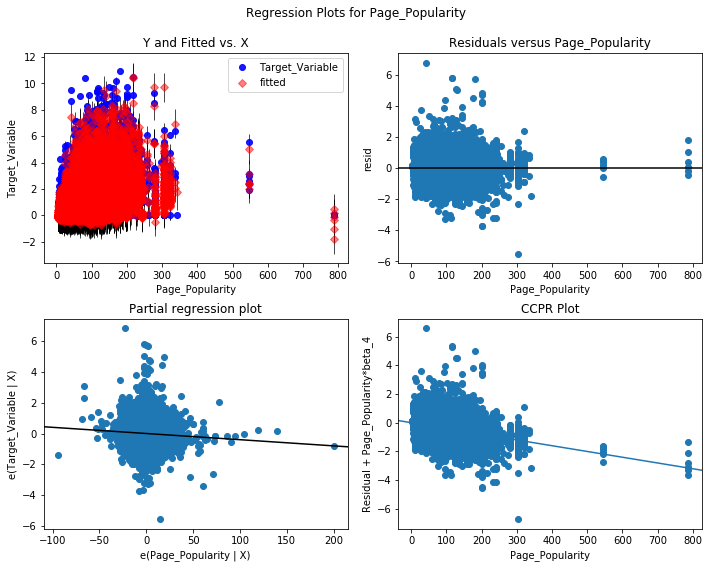
\includegraphics[width=.8\columnwidth]{../Figures/prp_complex_5}
	\caption{Plots on predictor: Page popularity.}
	\label{fig:prp_complex_5}
\end{figure}
%

\end{document}          
